\documentclass[12pt]{article}
\usepackage[utf8]{inputenc}
\usepackage[T1]{fontenc}
\usepackage[hidelinks]{hyperref}
\usepackage{biblatex}
\usepackage{graphicx}
\usepackage{xcolor}
\usepackage{hyperref}
\usepackage{parskip}
\usepackage{enumitem}
\usepackage{listings}
\usepackage[toc,page]{appendix}
\usepackage[section]{placeins}
\usepackage{wrapfig}
\usepackage{textcomp}

% Remove image float %
\usepackage{float}

% Cite all references %
\nocite{*}

\newcommand\todo[1]{\textcolor{red}{TODO : #1}}

\title{Mémoire}
\author{Rémy Pocquerusse}
\date{October 2017}

\addbibresource{references.bib}

\begin{document}

\maketitle

\par\hfil\null\par
\par\hfil\null\par
\par\hfil\null\par

\begin{center}
{\huge L'utilisation de l'intelligence artificielle pour la lutte contre la désinformation}
\end{center}

\clearpage

\renewcommand*\contentsname{Sommaire}

\clearpage

\tableofcontents

\clearpage

\section{Introduction générale}

Durant mon stage de Master 1, j'ai effectué une mission qui tournait autour d'une problématique simple : donner la possibilité à un utilisateur de décrire une chose et comprendre l'objet de cette chose côté machine. Plus précisément il me fallait catégoriser un texte pour pouvoir ensuite le classifier (parle t-on de science, d'écologie ?, etc.). Quelques pistes m'ont été données pour commencer mes recherches, notamment le traitement du langage naturel avec les possibilitées liées au web sémantique. C'est en explorant les ambitions du web sémantique que je me suis aperçu des enjeux d'un web ouvert aux données. En formulant des requêtes en langue naturelle ou structurée (type SQL) il est possible de récupérer des données formatées et liées, exploitables par une machine. Avec l'engouement pour l'intelligence artificielle qui a explosé grâce au big data \cite{sh}, la donnée est devenue précieuse. Beaucoup de problématiques de calcul et d'apprentissage tournent autour de la donnée. Dans le machine learning par exemple il faut des données fiables, structurées et en grande quantité. La création de dataset prend du temps et nécessite souvent une intervention externe du fait de la quantité de données à traiter manuellement. Par exemple ClaimBuster (outil que nous présenterons plus tard), a nécessité 3 mois de travail et 226 participants pour créer un dataset viable \cite{hassan2015quest}.
\\*
Pourtant ces données sont disponibles sur le web. N'y aurait-il pas un moyen de réduire ce temps de 3 mois au temps d'une simple requête ?

C'est à une de ces problématiques que le web sémantique (dont nous détaillerons le fonctionnement plus tard) tente aujourd'hui de répondre. Le web sémantique avec l'intégration de la sémantique dans le web vise à donner du sens aux données. Le mot Socrate ne réfère plus à un simple mot mais à un nom, à une personne qui possède une date de naissance, une nationalité, etc. Chaque donnée va référer à un objet qui possède des attributs universels qui le décrivent \cite{schemaPerson}.
\\*
Le web sémantique a déjà eu un impact important sur le web mais méconnu, ce qui peut s'expliquer par le fait qu'il est souvent défini comme un outil fait par des scientifiques pour des scientifiques \cite{semantic_web_has_failed}.
\\*
Un des cas les plus importants (et visible) est l'intégration de la sémantique dans le système de recherche de Google. Cela se traduit par des informations organisées à l'écran comme les infoboxes (panel situé à droite qui détaille notre recherche) ou encore des réponses directes aux recherches, exemple : \enquote{Quel est le vrai nom de molière ?} va nous afficher directement la réponse.

Le web sémantique a ouvert toutes sortes de données autour de différents thèmes : la médecine, le e-commerce, etc. La plupart des CMS permettent à leurs utilisateurs de structurer leurs données et de les ouvrir au reste du monde.
\\*
En médecine on peut noter \href{http://bio2rdf.org/}{Bio2RDF}, projet open source qui regroupe plus de 11 milliards de données liées relatives aux sciences de la vie et à la recherche clinique. On peut aussi citer DBPedia qui est une référence dans le domaine du web sémantique et qui s'est fixé pour but, depuis 2007, de produire des données liées avec des informations extraites de wikipédia.

Toutes ces données sont facilement maniables et interconnectables. Elles offrent des datasets gigantesques et hétérogènes directement exploitables par la machine. Cela permet de résoudre de nombreux problèmes d'apprentissage et de faciliter leur implémentation. Dans le cas présent nous allons voir comment ces données sont utilisées et pourraient être utilisées pour lutter contre la désinformation.

\subsection{La désinformation}

\enquote{La désinformation est un ensemble de techniques de communication visant à tromper des personnes ou l'opinion publique pour protéger des intérêts (privés ou non) et/ou d'influencer l'opinion publique.} \cite{wiki:desinformation}

La désinformation est donc un acte conscient et intentionnel ayant pour but de nuire à un groupe de personnes ou d'orienter son opinion. Elle peut se traduire par de la propagande, du prosélytisme ou de la manipulation sur tout type de sujet. Elle peut prendre tout type de configuration, mais prend souvent la forme d'allégations alarmantes ou révoltantes qui vont frapper le lecteur. Le but est de susciter une émotion forte pour que le lecteur s'empresse de partager l'information. Un mensonge plus frappant qu'une vérité se diffusera plus vite et plus loin avec un impact plus important. On estime par exemple, que sur twitter, une fake news a 70\% de chance en plus d'être partagée qu'une autre information \cite{vosoughi2017rumor}. 
Ainsi la désinformation se traduit plus généralement par une tentative de manipulation de l'opinion publique (exemple \href{https://www.20minutes.fr/societe/2261439-20180426-video-evacuation-tolbiac-retour-naissance-fake-news}{ici}) en transmettant des informations partiellement erronée (il est plus facile de croire à un mensonge enrobé de vérité). 

Il faut tout de même différencier la désinformation politique dont sont à l'origine des grandes organisations ou des états (on parle souvent de propagande) de la désinformation économique qui touche plutôt au buzz et à toute forme de reconnaissance (réseaux sociaux, etc.).

\subsection{Fake news}

Sur internet quand on parle de désinformation, on parle de fake news ou fausses nouvelles. On définit une fake news comme étant une information dont le but est de tromper consciemment un lecteur. Une fake news peut donc être définie comme étant une tentative de désinformation mais qui pour la plupart visent à induire en erreur et créer du buzz autour d'un fait. Elles sont particulièrement présentes sur les réseaux sociaux et dans les usines à clics. Mais on les retrouves aussi dans la presse spécialisée ou encore dans les médias politisés dont le but est la propagation de fausses informations pour servir leurs intérêts (retouche d'image, etc.).  

Un article faux n'est pas forcément une fake news tant qu'il n'y a pas l'intention de tromper, l'article peut avoir des fins humoristiques ou satiriques par exemple.

Une information se base sur un fait réel et donc vérifiable. Afin d'identifier une information comme étant fausse il faut pouvoir le prouver factuellement. Il est donc important de connaître l'existant (un ensemble d'informations vraies) pour pouvoir identifier une information fausse. Ici le but n'est pas de lutter contre ou éradiquer les fake news (cela reste de la liberté d'expression, dans une certaine mesure). Nous chercherons simplement à les identifier.

\paragraph{Contexte}

Même si le phénomène des fake news existe depuis longtemps, ce n'est que récemment, avec la campagne présidentielle américaine de 2016 et l'ingérence russe, qu'il a pris de l'ampleur. C'est à ce moment que l'on s'est vraiment rendu compte que toutes ces informations qui circulent sur internet ont un impact important sur le monde. Par exemple, en juillet 2016, le site wtoe5news a rapporté que le pape François avait approuvé la candidature à la présidence de Donald Trump. Cette information a été partagée plus d'un million de fois sur Facebook. A aucun moment il n'est mentionné le fait que wtoe5news est en fait un site d'informations satiriques. Ces fausses nouvelles se sont propagées au travers des sites d'informations et des réseaux sociaux, notamment Google, Twitter et Facebook. La tendance des utilisateurs à se servir des réseaux sociaux comme source d'information fait que n'importe qui s'improvise journaliste. Et qui s'improvise journaliste peut s'improviser propagandiste. En 2016, 62\% des adultes résidants aux États-Unis utilisent au moins parfois les réseaux sociaux pour s'informer. Malgré les retombées médiatiques suite à l'ingérence russe, ils sont 67\% en 2017 \cite{news_across_platforms_2017}.

Il est important de savoir quel impact peut avoir une fausse information lorsqu'elle est vue par des millions de personnes. Durant l'élection, une personne a été confrontée en moyenne à 3 fake news qui ont pu altérer son jugement \cite{allcott2017social}. De plus il est démontré que cette exposition à la désinformation a en partie influencé les résultats de l'élection présidentielle. Les fake news les plus partagées favorisaient l'élection de Trump. En moyenne une campagne de télévision a un impact de 0.02\% sur les votes d'une élection \cite{spenkuch2016political}. Si une fake news est aussi persuasive qu'une campagne de télévision on peut clairement dire que les fake news ont joué un rôle, déterminant ou non, dans l'élection de Trump.

\paragraph{Pourquoi favoriser leur détection plutôt que leur éradication ?} A cause de l'impact sur le monde réel que cela peut avoir. Susciter une vive émotion dans l'opinion publique est une des finalités de la fake news. Cela peut avoir des conséquences graves sur les évènements qui se déroulent (réponse par la violence, la haine). C'est un constat encore plus vrai en temps de guerre ou durant des périodes sensibles.

Cependant, cela reste de la liberté d'expression, s'il faut censurer toute personne ou site d'informations dès que l'on parle ou propage une fausse information (qu'elle soit satirique ou non), le sentiment de liberté sur internet s'en verra affecté. C'est pourquoi le but n'est que la détection de fake news, informer le lecteur qu'il consulte une fausse information.

\paragraph{Initiatives contre les fake news}

Les États, au vu de l'impact de la désinformation réagissent par la mise en place lois visant à contrer les fake news, en France mais aussi en Allemagne, Australie, etc. La faute incombe aux médias, ceux qui favorisent et ne modèrent pas les fausses informations ou les contenus haineux peuvent recevoir une amende \cite{allemagne_fake_news}. Le but étant de faire réagir les réseaux sociaux et sites de news.

Les États tentent aussi de sensibiliser la population aux dangers liés aux fausses informations et les invitent à toujours avoir un oeil critique sur les informations qui circulent \cite{haciyakupoglu2018countering}.

Le combat contre les fake news se déroule principalement sur les plateformes concernées et demeure avant tout une guerre technologique. C'est un travail trop conséquent pour être fait par des humains. Le but est donc de savoir comment détecter automatiquement une fake news. 

\subsection{Fake news et intelligence artificielle}

Comment l'intelligence artificielle peut-elle aider à la détection automatique de fake news ? 

Il existe différents outils qui intègrent de l'intelligence artificielle dans leur système pour agir sur les différentes étapes de la détection d'une fake news. Nous allons commencer par définir un processus simple d'évaluation de la véracité d'une fake news (voir Figure \ref{fake_news_process}).

\begin{figure}[ht]
\centering
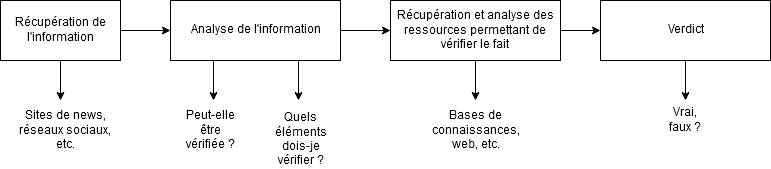
\includegraphics[width=\textwidth, draft=false]{diagrams/fake_news_process.png}
\caption{Processus de détection d'une fake news}
\label{fake_news_process}
\end{figure}

L'analyse du fait à vérifier et des ressources permettant de le vérifier, sont des étapes qui font appel aux techniques d'apprentissage de la langue mais aussi de la machine. Des solutions hybrides existent et permettent d'étendre le traitement de la langue en y ajoutant une dimension plus factuelle et réelle \cite{conroy2015automatic}.

Pour analyser un fait, nous avons une approche qui repose sur le traitement automatique du langage naturel (TALN). Le but de cette approche est d'analyser le texte brut pour identifier des patterns qui montrent qu'un texte est trompeur; lorsque le langage est trop négatif ou laisse transparaître des émotions trop vives; lorsque les mots utilisés sont similaires à ceux utilisés dans de précédentes analyses positives. Ces variations du discours ont conduit des travaux qui ont permis d'analyser les changements linguistiques d'un discours lorsque celui-ci est faux \cite{markowitz2014linguistic}. Le langage a tendance à être plus superficiel, moins descriptif, moins complexe etc. Beaucoup d'indices permettent d'établir un verdict. 
\\*
Cette approche est en revanche trop peu déterminante et trop peu certaine. Elle est utilisée principalement pour complémentariser des approches plus sophistiquées. En effet pour détecter et prédire la tromperie il est nécessaire d'utiliser des structures syntaxiques plus avancées et des preuves factuelles. L'analyse syntaxique profonde (deep syntax) va permettre de construire des ensembles de règles permettant de décrire la structure syntaxique d'un texte. Appliqués à un texte, ces ensembles de règles vont permettre d'identifier des patterns plus évolués permettant une détection plus précise et certaine des cas de tromperie \cite{feng2012syntactic} \cite{collinsprobabilistic}.

Les méthodes d'analyse linguistiques sont innombrables et s'intéressent toutes à identifier des patterns différents. Il s'agit plus de détecter le mensonge que de le prouver. Il est donc nécessaire de coupler ces approches avec des méthodes qui vont prouver factuellement que le fait est vrai ou faux.

C'est ici que le web sémantique va jouer un rôle prépondérant. Les bases de connaissances (ou Knowledge Base, abrégé KB) vont apporter un contexte sémantique aux données. Une KB va représenter le monde en attribuant aux données des propriétés qui vont la décrire. Ainsi lorsque je veux savoir si Barack Obama est allé à Harvard, je vais étudier les relations qui existent dans ma base entre l'entité Barack Obama et Harvard pour établir un verdict. Nous verrons en détail des méthodes qui utilisent cette approche dans la section \ref{section_knowledge_graph}.

Le machine learning est aussi une approche viable. L'outil de fact-checking ClaimBuster par exemple va utiliser le machine learning pour identifier des patterns de phrases pouvant contenir des faits à vérifier. Cela permet d'identifier dans un texte les phrases qui nécessitent une vérification. 
\\*
On a aussi des moyens plus complémentaires comme la simple vérification de la source émettrice de l'information (ce qui aurait pu empêcher la propagation de la fake news sur l'implication du pape dans la campagne  de Donald Trump). Il est aussi possible d'établir un score de confiance sur les sources d'information en fonction des expériences passées : ce sont souvent les mêmes sources qui propagent de fausses informations.

D'autre part, l'analyse des médias utilisés dans un article peut conduire à détecter de potentiels cas de fake news : si un article de 2017 présente des images d'une manifestation violente, on va rechercher des informations sur ces images. Sur google image il est possible d'effectuer une recherche par image et ainsi déterminer la date de la première apparition d'une image sur le web. Si une image datant de 2012 se retrouve sur un article de 2017, alors c'est une possible tentative de désinformation (exemple \href{https://www.lemonde.fr/les-decodeurs/article/2017/10/02/violences-policieres-en-catalogne-attention-aux-images-trompeuses_5194905_4355770.html}{ici}). Il est aussi possible de déterminer si une image a été altérée et retouchée \cite{krawetz2007picture}.

L'intelligence artificielle a un rôle prépondérant à jouer dans la détection de fake news. Elle intervient à toutes les étapes. Principalement dans le TALN mais aussi dans la façon de traiter l'information (machine learning).

Pour conclure, nous avons vu que les méthodes liées à l'analyse syntaxique vont se construire autour du TALN et de modèles statistiques tandis que celles sur les KBs vont regrouper des méthodes orientées sur la théorie des graphes. Mais ces deux approches sont complémentaires. L'analyse syntaxique va permettre à la KB d'identifier les données qu'elle manipule et de les structurer. Inversement la KB va permettre à l'analyse syntaxique d'ajouter une dimension concrète et matérielle aux données. Et permettre ainsi de replacer la donnée dans l'existant. D'autres méthodes permettent d'étendre ces approches et s'avèrent essentielles pour un système de fact checking autonome (si un article est vrai mais présente des images trompeuses, il est nécessaire de s'en rendre compte).

On discerne donc ici deux approches, l'une qui va tenter d'analyser le fait énoncé et rechercher un argumentaire sur le web en appliquant des algorithmes de TALN pour construire un verdict. Et l'autre qui va se baser sur des données issues du web, déjà structurées et formatées, pour établir son verdict.

\subsection{Fact-checking}

Le fact-checking ou vérification de faits représente l'acte de vérifier la véracité d'une assertion. Il s'agit de traiter l'information afin de démêler le vrai du faux, du partiellement vrai du partiellement faux. Il est apparu aux États Unis dans les années 2000. Le fact checking est considéré aujourd'hui comme une forme de journalisme à part entière \cite{lemonde_fact_check_nouveaute_journalistique}. Avec la montée des réseaux sociaux et la propagation toujours plus rapide et massive l'information, le fact checking a pris de l'ampleur récemment. De plus en plus de site d'informations se munissent de leurs propres laboratoires de fact checking \cite{memoire_fact_check_nouveaute_journalistique}. 

Mais les sources d'information sont innombrables et le flux de données journalier est tel qu'il est impossible de vérifier chaque information manuellement. Que ce soit sur des blogs, les réseaux sociaux, les sites d'informations, etc. filtrer l'information et la vérifier représente un temps de travail important. Les sites peuvent apporter leur propre système de fact checking humain (voir \href{http://decodeurs.blog.lemonde.fr/}{ici}) mais le nombre de faits couverts reste très limité.

\paragraph{Fact-checking : les limites}

Le fact-checking est un travail qui est chronophage, en effet il faut tout d'abord trouver et identifier les faits vérifiables et dignes d'intérêt. Il y a ensuite un travail de recherche pour comprendre le fait et le vérifier en faisant attention à ne pas tomber soi-même dans le piège de la désinformation. Cela signifie confronter et vérifier ses sources. 
Tous ces critères font qu'entre le moment ou une déclaration est faite, et celui ou elle est vérifiée s'écoule un certain laps de temps, qui peut éventuellement rendre le fact-checking inutile si la déclaration a déjà eu l'impact voulu.

\paragraph{Quels objectifs ?}

L'objectif derrière le fact checking reste actuellement très politique, il s'agit de traquer les mensonges de personnalités influentes.

Mais à terme le fact checking doit permettre de toujours manipuler une information avérée et sûre quelle que soit sa source ou sa forme.

Il n'existe actuellement aucun système universel, 100\% automatisé et 100\% fiable qui permette de réaliser des opérations de fact-checking sur tout type de support. La finalité d'un système de fact-checking serait tout d'abord d'être capable de caractériser, classifier et comprendre l'information pour ensuite vérifier sa légitimité. 

\paragraph{Système entièrement autonome ou du moins le plus possible}

Quelles seraient les tâches d'un système entièrement autonome ? Quelle est la faisabilité de chacune de ces tâches ? Quelle marge d'erreur est-on prêt à accepter avant de définir notre système comme entièrement autonome ? Enfin, confier à un système informatique autonome la responsabilité de vérifier des faits revient à demander à une machine de faire du journalisme. Cela peut poser des problèmes éthiques, peut-on faire confiance à une machine pour nous dire ce qui est vrai ou faux ?

Un tel système doit pouvoir extraire une assertion d'une source et la vérifier sans intervention humaine et dans un temps raisonnable. Pour cela il doit pouvoir se "nourrir" de différentes sources d'information qu'il va confronter. Plusieurs challenges importants entrent en compte dans la vérification d'un fait.

\paragraph{Challenges}

Comme nous l'avons précisé pour qu'un fait soit analysé il faut tout d'abord qu'il soit compris. Il faut donc faire comprendre au système le langage humain, c'est le TALN. C'est un domaine vaste qui fait appel à de nombreux sous domaines dans le traitement du langage comme l'analyse syntaxique ou l'analyse sémantique. Bien que très avancée, cette science est en revanche loin d'être parfaite \cite{nlp_not_perfect}.

Mais un système aussi performant soit-il ne fonctionnera pas sans données fiables. Il faut pouvoir trouver et collecter ces données pour alimenter le système. Les sources de données structurées et utilisables sont innombrables, que ce soit avec le développement du web sémantique, du linked-data, des bases de connaissances, des apis de type REST et de l'open data on possède déjà des sources de données conséquentes et fiables. On a ensuite des sources de données plus génériques, moins ordonnées mais tout aussi exploitables. Je parle ici des sites d'informations et plus généralement de toutes les informations disponibles sur internet : réseaux sociaux, etc. Ce sont des sources de données plus ou moins fiables mais la quantité d'informations produites par ces sources est considérable. Ces sources peuvent être interrogées via des outils de type web scraping et data mining.
Toutes ces sources de données peuvent être confrontées pour permettre de chercher et étoffer un fait pour pouvoir le comprendre et le vérifier.
Mais les sources de données ne se limitent pas à ce que l'on trouve sur internet.

On identifie donc 3 sources de données différentes, les données : 

\begin{itemize}
    \item Déjà traitées par des sites spécialisés ou communautaires : beaucoup de sites d'informations ont développés leurs propres systèmes de fact-checking (tous manuels). 
    \item Structurées ou semi-structurées : issues de l'open data, ou d'api telles que wikimédia
    \item Non-structurées : issues de toutes sources potentiellement utilisables
\end{itemize}

Les données non structurées peuvent se trouver directement dans la vie réelle à travers différents médias : les chaînes de télévision, les émissions de radio (mais aussi les journaux, magazines), etc. Tout signal vidéo ou audio est potentiellement une source intéressante pour le système. Il faut pouvoir interroger et structurer ces sources : savoir qui parle, dans quel contexte.

Une fois ces informations structurées nous devons savoir lesquelles définissent des faits réels et vérifiables. Filtrer les informations en fonction de la vérifiabilité d'une assertion. C'est-à-dire éliminer toute phrase qui définit une opinion, de l'humour, de l'ironie, figures de style, etc. et bien sûr les phrases lambda. De plus comment détecter qu'un fait se construit sur plusieurs phrases ? Comment construire un argumentaire appuyé par des preuves concrètes qui permettent de remettre en cause le fait.

Enfin, une fois le fait collecté et défini comme vérifiable, il faut pouvoir construire un argumentaire qui va permettre de juger ce fait. Même si l'on arrive à collecter les informations autour du fait, comment va t-on les organiser et les interroger ? Comment s'assurer que l'on travaille avec des données fiables lorsqu'elles sont extraites de sources non fiables ? 

\subsection{Objectifs}

J'ai choisi ce sujet car il fait appel à des techniques et des domaines de recherches très nombreux que j'ai souvent survolés : web sémantique et linked-data, analyse sémantique, bases de connaissances, traitement automatique du langage, machine learning, knowledge graph, web scraping, web crawling, data mining, etc. Ce sont des sujets très variés mais qui mis bout à bout pourraient amener les systèmes de fact-checking à évoluer vers d'autres approches. 

Pour vérifier un fait, un système de fact-checking va analyser l'information et les ressources disponibles sur le web de façon automatique, la cartographier et tenter de la comprendre. Analyser toutes les données disponibles pour en comprendre le sens, et construire des modèles cohérents permettant de structurer l'information pour élaborer des modules basés sur des algorithmes d'apprentissage efficaces. C'est-à-dire récupérer des informations complexes, les structurer et construire des algorithmes issus de ces données par apprentissage supervisé. La finalité de ces algorithmes pourrait être multiple : détection de fake news, détection d'image, etc. L'enjeu derrière un web structuré est vital pour l'évolution du fact-checking mais aussi de l'intelligence artificielle. Cela permet de travailler avec des sets de données complexes et conséquents.

C'est un objectif très vaste voir impossible. Mais pour lutter contre la désinformation et arriver à un système de fact checking efficace et autonome c'est une approche qu'il faut évaluer.

Le but de ce mémoire est d'étudier différentes approches utilisées dans le fact checking automatique pour pouvoir proposer des évolutions vers un système viable et cohérent. Au travers de ce problème de fact-checking, nous verrons que deux choses sont primordiales : une source de donnée conséquente et fiable et un moyen d'interroger et comprendre cette source de donnée.

\section{Outils et techniques}

\subsection{Web sémantique}

\enquote{To a computer, the Web is a flat, boring world, devoid of meaning. This is a pity, as in fact documents on the Web describe real objects and imaginary concepts, and give particular relationships between them. For example, a document might describe a person. The title document to a house describes a house and also the ownership relation with a person. Adding semantics to the Web involves two things: allowing documents which have information in machine-readable forms, and allowing links to be created with relationship values. Only when we have this extra level of semantics will we be able to use computer power to help us exploit the information to a greater extent than our own reading.} - \textit{Tim Berners-Lee "W3 future directions" keynote, 1st World Wide Web Conference Geneva, May 1994} \cite{tim}

Revenons en au web sémantique afin de clarifier quelques termes et approfondir son mode de fonctionnement. Cela nous permettra de mieux comprendre tous les outils liés à la sémantique comme les knowledge graph. Actuellement la navigation et la recherche d'information sur le web nécessitent une action humaine. Une machine n'est pas encore capable de rechercher et d'analyser efficacement des données sur le web. La collecte de données automatique est possible mais la machine ne peut déterminer de manière fiable le type d'entité, les thèmes, les relations, le contexte, etc... des données qu'elle manipule.
\\*
Les aspirations du W3C sont de créer un web exploitable par des machines en le transformant en une base de connaissance géante.
La navigation sur le web est possible via des hyperliens, cependant elle doit aussi pouvoir se faire au niveau de données structurées pour que les machines puissent exploiter de façon plus efficiente et précise les données contenues sur le web.

Le web sémantique ou web 3.0 est une extension du web, standardisée par le W3C. Ces standards recommandent l'utilisation de format de données et de protocoles normés, plus généralement il s'agit du RDF (Resource Description Framework).

\subsubsection{RDF}

Le RDF (Ressource Description Framework) est un modèle de description des données permettant l'échange entre différentes applications. Il permet la structuration, l'indexation et la standardisation des données disponibles sur le web. Un schéma simple est utilisé pour structurer les échanges et les relations entre les ressources (documents, personnes, concepts abstraits...). Sachant qu'une ressource est représentée par une IRI (International Resource Identifier), par définition unique, il est possible de lier différentes ressources entre elles en utilisant un triplet : <Subject, Property, Object> ou Subject et Object sont définis par des IRI. La propriété d'une relation spécifie la nature du lien entre les 2 ressources : isChildOf, diedIn... Pour spécifier ces relations, le RDF utilise le langage XML (ou RDF/XML) \cite{rdf}. C'est ce qu'on appel des données liées au linked-data.

Ainsi le web sémantique ressemble à un graphe géant regroupant plusieurs milliards de liens (triplets) permettant une navigation et une interrogation des données plus efficaces. En respectant le RDF, une entreprise, une université ou n'importe quelle entité peut ouvrir ses données au web afin qu'elles soient exploitables par n'importe quelle machine.

Le RDF permet l'utilisation de différents "vocabulaires" ou ontologie pour traiter les données. Il pourrait être comparé à une grammaire et une ontologie à son vocabulaire. Par exemple FOAF (Friend Of A Friend) est une ontologie permettant la structuration de personnes. \cite{foaf}

\subsubsection{Ontologie}

Une ontologie permet de représenter les connaissances en les organisant sous forme de classes, de relations, de règles (ou implication) etc... Le but ici est de structurer les informations collectées sur le web.

Une ontologie se structure en essayant de comprendre le monde : comment est structuré notre monde, par quels concepts est-il défini ? Quelles sont les relations entre ces concepts permettant d'expliquer notre monde. Une ontologie ne s'intéresse donc par à ce qui est possible ou ce qui pourrait être mais s'intéresse à ce qui est. \cite{shirky} \cite{schema}

Toutes ces règles, conventions, standards et vocabulaires ont pour objectif de normaliser l'échange de données liées au web afin de construire un web dans lequel les ressources sont identifiables non par des urls mais par des données. Ainsi deux sources de données différentes qui utilisent les mêmes ontologies peuvent fusionner sans problèmes, et l'interrogation distincte de ces sources se fait avec les mêmes requêtes.

Par exemple, comme dans la figure \ref{fig1}, et via The Open Graph protocol (OGP) il est possible d'intégrer des balises HTML qui vont ajouter de la sémantique à un objet \cite{ogp}. Cela permet de rendre cet objet interopérable. Il pourra être ensuite traité de façon complexe avec d'autres objets.

\begin{figure}[ht]
\centering
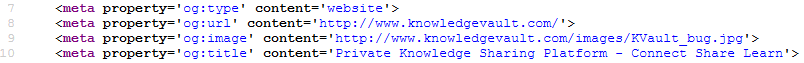
\includegraphics[width=\textwidth, draft=false]{imgs/og_example.PNG}
\caption{Exemple d'utilisation de l'open graph dans le code source d'une page : \url{http://www.knowledgevault.com/}}
\label{fig1}
\end{figure}

Ces données peuvent ensuite être collectées pour être rassemblées et raffinées dans des bases de connaissance telles que Yago.

\subsubsection{Exemple : Yago}

Une KB (knowledge base ou base de connaissance) est une base de données utilisée pour stocker et structurer du contenu lié à un domaine spécifique afin qu'il soit exploitable par une machine. Une KB lie ses données entre elles en y appliquant des règles, des faits ou des prédicats. A partir de ces constats, la KB peut déduire et faire évoluer la structuration de ses données. Prenons un exemple simple, j'ai une ontologie qui décrit les relations entre les personnes. En particulier cette ontologie me dit que si 2 personnes ont une même mère alors elles ont une relation fraternelle. Ainsi si j'enregistre 1 personne, ici la mère, et que je lui attribue un lien de maternité avec deux autres personnes, ma base sera capable de créer automatiquement un lien de fraternité entre ces 2 personnes.

Certaines KB ont pour but d'exploiter les données du web sémantique, la plupart se cantonne néanmoins, pour le moment, à la structuration des données présentes sur des domaines spécifiques, notamment wikipédia. On peut citer par exemple \href{http://wiki.dbpedia.org/about}{DBpedia} ou \href{https://www.wikidata.org/wiki/Wikidata:Main_Page}{Wikidata}, ou d'autres encore qui tentent d'étendre leur champ d'action à d'autres sources comme \href{http://www.mpi-inf.mpg.de/departments/databases-and-information-systems/research/yago-naga/yago/}{Yago}.

Yago est une KB créée par l'institut Max-Planck d'informatique à Sarrebrück en 2008. Contrairement à DBpedia ou Wikidata qui s'appuient sur un effort communautaire, le but de Yago est d'extraire des données de sources différentes (actuellement Wikipedia et Wordnet). Tout cela automatiquement et en plusieurs langues. Beaucoup de KB comme Yago s'organise sous la forme de graphe. L'information dans ces bases est représentées par un graphe géant constitué de millions de triples. Ces graphes sont appelés graphes de connaissance.

Les KB comme Yago permettent d'interroger Wikipedia et différentes sources avec des requêtes précises, par exemple : "Les peintres français du 16ème siècle" ou "Les villes de Chine de plus d'un million d'habitants". Les requêtes après traitement se font en langage naturel et retourne des données structurée et formatée pour être utilisée directement avec le système. Yago regroupe actuellement des informations sur plus de 10 millions d'entité (personnes, villes, etc.) et plus de 120 millions de faits sur ces entités. 
Il existe de nombreuses bases de connaissances qui contiennent des données hétérogènes comme Yago mais d'autres se concentrent sur des domaines spécifiques comme la médecine (ex : Precision Medicine Knowledgebase). Ces bases apportent une matière essentiel à la lutte contre la désinformation, ce sont des sources de données fiables et dont le requêtage est facilement automatisable.
Le langage d'interrogation de ces données est le SPARQL.

Yago est disponible en open source \href{https://github.com/yago-naga/yago3}{ici}.

\iffalse
\subsubsection{SPARQL}

SPARQL (Protocol And RDF Query Language) est un langage de requête orienté données permettant d'intéragir avec des données RDF à travers le web. SPARQL permet de questionner le web sémantique, plus précisément les triplets, qui forme le graphe géant du web sémantique.

Exemples pour Yago (n'est plus accessible sur les SPARQL endpoints donc non testable pour le moment) :

Liste des prédicats associés à l'entité France.

\begin{lstlisting}[language=SPARQL, backgroundcolor=\color{lightgray}]
PREFIX rdf: <http://www.w3.org/1999/02/22-rdf-syntax-ns#> 
PREFIX yago: <http://yago-knowledge.org/resource/>
SELECT DISTINCT ?x WHERE {
    yago:France rdf:type ?x.
}
\end{lstlisting}

\iffalse
Savoir si l'entité France est référencée sur wikipedia.

\begin{lstlisting}[language=SPARQL, backgroundcolor=\color{lightgray}]
PREFIX rdf: <http://www.w3.org/1999/02/22-rdf-syntax-ns#> 
PREFIX yago: <http://yago-knowledge.org/resource/>
SELECT DISTINCT ?x WHERE {
    yago:France yago:hasWikipediaUrl ?x.
}
\end{lstlisting}

\fi

Autre exemple sur DBPedia, dans quelles catégories s'inscrit une voiture ?

\begin{lstlisting}[language=SPARQL, backgroundcolor=\color{lightgray}]
PREFIX dbr: <http://dbpedia.org/resource/>
PREFIX  dct:  <http://purl.org/dc/terms/> 

select ?categorie, (COUNT(?result) as ?numberResult) 
where {
   ?result dct:subject ?categorie.
   ?search rdfs:label "Voiture"@fr .
   ?search <http://dbpedia.org/ontology/wikiPageWikiLink> 
   ?categorie
} ORDER BY ?numberResult
LIMIT 1000
\end{lstlisting}

Tester \href{http://fr.dbpedia.org/sparql?default-graph-uri=&query=PREFIX+dbr\%3A+\%3Chttp\%3A\%2F\%2Fdbpedia.org\%2Fresource\%2F\%3E\%0D\%0APREFIX++dct\%3A++\%3Chttp\%3A\%2F\%2Fpurl.org\%2Fdc\%2Fterms\%2F\%3E+\%0D\%0A\%0D\%0Aselect+\%3Fcategorie\%2C+\%28COUNT\%28\%3Fresult\%29+as+\%3FnumberResult\%29+\%0D\%0Awhere+\%7B\%0D\%0A+++\%3Fresult+dct\%3Asubject+\%3Fcategorie.\%0D\%0A+++\%3Fsearch+rdfs\%3Alabel+\%22Voiture\%22\%40fr+.\%0D\%0A+++\%3Fsearch+\%3Chttp\%3A\%2F\%2Fdbpedia.org\%2Fontology\%2FwikiPageWikiLink\%3E+\%0D\%0A+++\%3Fcategorie\%0D\%0A\%7D+ORDER+BY+\%3FnumberResult\%0D\%0ALIMIT+1000&format=text\%2Fhtml&timeout=0&debug=on}{ici}

\subsubsection{Wikidata}

\todo{A mettre en forme et à intégrer sur un eexemple de fact checking}

Info : dans une entrée, si ns = 14, alors c'est une sous catégorie de l'objet recherché. Ici les requêtes sont limitées à 10 résultats.

Faire une recherche : 

\url{https://fr.wikipedia.org/w/api.php?action=query&list=search&format=jsonfm&srsearch=Panneau+solaire&utf8=1}

Rechercher une catégorie :

\url{https://fr.wikipedia.org/w/api.php?action=query&titles=Panneau+solaire&prop=categories&clshow=hidden&utf8=1}

clshow=hidden permet d'afficher les catégories cachées comme les portails qui sont bien plus génériques que les catégories.

clshow=!hidden permet de n'afficher que les catégories spécifiques de l'article, la recherche est bien plus simple.

Catégories liées aux Technologies :

\url{https://fr.wikipedia.org/w/api.php?action=query&list=categorymembers&cmtitle=Category:Technologie&utf8=1}

Catégories principales de wikipédia (portails, en anglais)

\url{https://en.wikipedia.org/w/api.php?action=query&list=categorymembers&cmtitle=Category:Main%20topic%20classifications&utf8=1}

Plus d'infos : 

\url{https://www.mediawiki.org/wiki/API:Categories}

\url{https://m.mediawiki.org/wiki/API:Query#Generators}
\fi

\subsubsection{Conclusion}

Le web sémantique est une source de données interopérable qui traite des données complexes. La donnée représente un objet, cet objet a des relations, des attributs et des propriétés. Mis bout à bout ces objets permettent d'avoir une représentation concrète de la réalité dans un ou plusieurs domaines. C'est cet ancrage dans la réalité qui donne au web sémantique le contexte qui manque aux données brutes. Les données liées sont primordiales pour faire évoluer le fact checking vers des approches plus performantes et fiables.

\subsection{Claimbuster}

Nous allons maintenant étudier un des outils les plus évolués en matière de fact-checking automatique. Cette étude va nous permettre de mettre en lumière les enjeux et challenges pour aboutir à un système autonome.

\subsection{ClaimBuster} 

ClaimBuster est ce qu'on appelle un Fact checking system \cite{hassan2015quest}, c'est-à-dire un système qui va procéder de manière automatique, du moins en partie, à une ou plusieurs étapes de vérification d'un fait. Ce système permet d'extraire des faits d'une source de données et de leur appliquer un score qui détermine si un fait est plus ou moins vérifiable. ClaimBuster est utilisé pour faciliter le processus de vérification de fait, il a pour fonction d'aider le journaliste dans son travail. Cet outil va permettre au journaliste de se concentrer sur la vérification d'un fait plutôt que sur son identification et son extraction. ClaimBuster est spécialisé dans la vérification de faits liés à la sphère politique.
\\*
Il se construit autour de différentes techniques d'apprentissage et de traitement de données : l'apprentissage automatique (machine learning), le traitement automatique du langage naturel, etc. \cite{hassan2017claimbuster}.
De plus, il peut requêter des sources de données automatiquement (web ou audio). Il est aussi capable, sur certains faits, d'appliquer automatiquement un état qui définit si un fait est plus ou moins vrai. Pour ce type de scénario, ClaimBuster dispose de deux méthodes pour vérifier un fait. 

Soit il va questionner des sources de données de faits déjà vérifiés et dans ce cas il ne se présente que comme une interface entre le fait et sa vérification. Dans le second cas il est capable de produire un verdict en traduisant le fait en question. Il requête ensuite des systèmes de type questions-réponses (exemple : Google), compare et confronte les résultats pour établir son verdict. Dans certains cas, ce système est donc entièrement autonome.

\begin{figure}[ht]
\centering
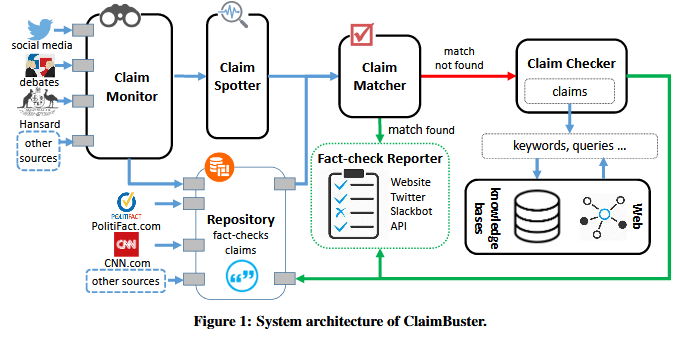
\includegraphics[width=\textwidth, draft=false]{imgs/claimbuster.PNG}
\caption{Architecture de ClaimBuster}
\label{claimbuster}
\end{figure}

\paragraph{Claim Monitor}

C'est le module qui recherche et récupère les données. Au travers de différentes sources de données il va rechercher des textes à analyser. Ce module travaille sur trois différentes sources de données. Il y a d'abord la nécessité de travailler sur des informations en live afin de pouvoir instantanément évaluer les propos d'une personne : les débats politiques par exemple. C'est pour cela que les médias audiovisuels sont une importante source de données. ClaimBuster utilise différentes api pour traduire ce flux en données utilisables, notamment la structuration des données au travers de l'identification de l'orateur \cite{joseph2015speaker}. Ensuite le Claim Monitor travaille sur les données disponibles via les réseaux sociaux, il suit 2220 comptes Twitter appartenant à différents types d'entité (personnalité politique, médias d'information, etc.). Seul les tweets relatifs à la politique sont gardés. Enfin ce module récupère diverses informations issues de plusieurs sites web.

\paragraph{Claim Spotter}

Une fois l'information captée et filtrée, on se retrouve avec des données liées à la politique et potentiellement constatables. Actuellement l'élément de ClaimBuster le plus mature est le Claim Spotter qui va attribuer un score à une assertion en fonction de la capacité du fait à être vérifié : proche de 1, le fait peut être vérifié, proche de 0 le fait n'est pas vérifiable. Ce module a été construit autour d'un modèle défini par plusieurs dizaines de milliers de faits vérifiés manuellement. La précision de ce modèle est de plus de 80\%. Le processus peut éventuellement s'arrêter à cette étape si les étapes suivantes n'apportent pas d'informations concluantes. Dans ce cas on va simplement retourner à l'utilisateur une suite de faits définis comme vérifiables et leurs scores.

Le Claim Spotter et l'identification des faits potentiellement vérifiable s'est fait au travers du machine learning et l'apprentissage supervisé. Le set de données est composé de plusieurs dizaines de milliers de phrases prononcées durant des discours, débats, etc. politiques. Chaque phrase est identifiée comme étant plus ou moins importante et plus ou moins vérifiable. Plus précisément on différencie les : 
\begin{itemize}
    \item NFS (Non Factual Sense) : qui sont des phrases banales décrivant des opinions, des traits d'humour, etc. 
    \item UFS (Unimportant Factual Sentence) : représente des phrases qui décrivent des faits qui n'ont que peu d'importance, ex : "Demain il va pleuvoir"
    \item CFS (Check-worthy Factual Sentence) : des phrases dignes d'intérêts, qui valent la peine d'être vérifiées. 
\end{itemize}

Les algorithmes sont entraînés par apprentissage supervisé, c'est-à-dire que l'on va travailler sur des données annotées, déjà évaluée. Les algorithmes de machine learning vont emmagasiner ces données et apprendre de ces données. Ils vont ensuite être capable d'évaluer un fait en se basant sur leur expérience pour déterminer s'il est vérifiable ou non.

Afin de noter et classifier ces phrases, ClaimBuster va utiliser des Support Vector Machines (SVM), en français, séparateurs à vaste marge. Les SVM sont une classe d'algorithmes d'apprentissage supervisé destinés à la prévision de variable qualitative binaire, c'est-à-dire des problèmes de discrimination : un fait est vrai ou faux. Plus précisément, si l'on prend une phrase de type CFS, on va la traiter comme étant positive (les autres types étant négatifs). La SVM va ensuite trouver la marge optimale et tenter de trouver un classifieur permettant de généraliser et séparer les observations et ainsi leur attribuer un score distinctif.

\paragraph{Claim Matcher}

A partir de ce point, on ne travaille que sur des faits définis comme vérifiables, on a éliminé les opinions et tout ce qui n'est pas une assertion. Ainsi étant donné une phrase qui énonce un fait, on va essayer de prouver ou non sa véracité. Le Claim Matcher va tenter de trouver des faits déjà vérifiés (issus de plusieurs sites de fact-checking) et en rapport avec l'assertion. Pour cela il utilise deux méthodes : l'une consiste à simplement établir une concordance entre les mots utilisés pour qualifier le fait et ceux qui définissent les faits vérifiés; l'autre se base sur une analyse sémantique des faits \cite{rus2013semilar}. 
\\*
Si le fait n'est pas présent, alors le système va tenter de vérifier le fait automatiquement.

\paragraph{Claim Checker}

Le rôle de ce module est de construire un argumentaire autour du fait en collectant des informations additionnelles issues de bases de connaissances. Pour ce faire il va interroger la base de connaissance de \href{https://www.wolframalpha.com/about.html}{Wolfram Alpha} grâce à des questions générées automatiquement \cite{heilman2009question}. 
\\*
Par exemple si on a l'assertion suivante : "The largest country in the world is China", et que l'on recherche ceci sur Wolfram Alpha on n'obtient aucune donnée concluante. Mais si on entre ceci : "The largest country in the world", l'assertion va être interprétée comme une question (par l'absence de COD), et le résultat retourné est la Russie. Par confrontation, on peut voir qu'il existe une différence entre les résultats et donc le fait à des chances d'être faux. Faire du fact-checking entièrement automatisé sur des questions simples est donc faisable.

Ainsi Claim Checker va potentiellement arriver à un verdict s'il trouve des incohérences entre les différentes questions posées. Pour assurer une fiabilité plus poussée par un argumentaire plus fourni, on envoie les questions à Google et on analyse les premiers résultats.

\subsection{Cas d'essai}

ClaimBuster a été testé sur des cas d'essais concrets durant l'élection présidentielle américaine de 2016. Un total de 30737 phrases a été collecté sur les 21 débats qui on eu lieu entre août 2015 et avril 2016.
\\*
Sur ces 30737 phrases, ClaimBuster a détecté 776 réclamations factuelles du côté des républicains (5,06\%) et 484 (6,73\%) pour les démocrates. Par réclamation factuelle on entend fait vérifiable, soit un fait qui a obtenu un score de plus de 0,5 \cite{hassan2017toward}.

Durant les débats, différents organismes ont vérifié certaines assertions des candidats. Ces verdicts, 224 à partir de CNN et 118 à partir de PolitiFact ont permis de tester la fiabilité de ClaimBuster. La moyenne de ClaimBuster pour les phrases vérifiées par CNN est 0.433 comparée à 0.258 pour les phrases non sélectionnées par CNN, et sensiblement la même chose pour PolitiFact. Cela permet de démontrer l'utilité de ClaimBuster dans le processus de fact checking.

\subsection{Critique}

Plusieurs approches ont été utilisées pour attribuer des scores de vérifiabilité aux faits : SVM mais aussi Naive Bayes Classifier (NBC) ou encore Random Forest Classifier (RFC). SVM a été retenu du fait du haut taux de réussite (96\%, soit autant que les capacités d'analyse d'un être humain). Aucune ne se base sur le TALN, qui est ici défini comme loin d'être parfait. Mais le fait de construire son algorithme sur de l'apprentissage supervisé va rendre l'évolution de ClaimBuster bien plus compliquée. Si demain ClaimBuster souhaite étendre son activité de fact checking au-delà de la sphère politique, ce sont des dizaines de datasets qu'il faudra construire. Même chose s'il veut s'ouvrir à d'autres langages. Dans cette approche, l'utilisation du machine learning contraint le système à avoir un seul domaine de prédilection : la politique. En outre sans TALN, ClaimBuster ne comprend pas la sémantique du fait qu'il vérifie, cela limite son champ d'action et ses possibilités d'évolution. Sans comprendre à quoi se rapporte le fait, à quoi il fait référence, il est compliqué de construire un argumentaire fiable. Par exemple pour la phrase suivante : \enquote{The American Revolutionary War was a war fought between Great Britain and Russia}, ClaimBuster ne donne qu'un score de 0.32 soit un fait que l'on peut ignorer, qui n'est pas vérifiable ou ne vaut pas la peine d'être vérifié. Autre exemple : \enquote{Hayao miyazaki is dead.} ne donne qu'un score de 0.22. Mais ici ce sont des faits vérifiables et qui méritent d'être vérifiés. Pourtant Claimbuster les classe presque sur un pied d'égalité avec l'assertion suivante : \enquote{I love war} qui obtient un score de 0.17. Cela montre les limites du machine learning tel qu'il est utilisé par ClaimBuster.

Autre point, certaines étapes nécessaires à la vérification d'un fait semblent peu adéquates ou peu fiables. Le ClaimChecker, afin d'étoffer l'argumentaire, va rechercher des informations sur les premières pages de google. Cette étape est assez floue mais est-ce que simplement sortir des phrases de Google sans vérifier les sources ce n'est pas tomber dans le piège de la désinformation ? Comment construire un argumentaire efficace sans utiliser le TALN ? Cela est d'autant plus vrai lorsque l'on essaye de vérifier une information récente, qui change souvent ou qui est floue. Et ici encore, sans TALN, impossible de dire si l'information a un sens et est corrélée au fait. De plus, les sources ne sont pas vérifiées, aucun module ne permet d'assurer la fiabilité d'une source. Il est donc très probable de se retrouver à traiter des informations fausses.

Ces critiques faites, il faut quand même rappeler que le fact checking automatique n'en est qu'à ses débuts et ClaimBuster fait parti des pionniers. Trouver un mode viable est plus important que rechercher le graal en proposant directement un système parfait. Ici le but premier est d'aider le journaliste même si la finalité serait d'obtenir un système autonome. ClaimBuster se base sur les assertions de personnalités politiques. En se perfectionnant sur cette base il pourra peut être s'ouvrir à d'autres domaines. Avec le TALN, il est possible d'utiliser une approche qui sera peut être au début moins viable, en effet l'outil évoluera en fonction de l'évolution du TALN. Mais cet outil sera plus simple à ouvrir à tout type de domaines et langues. En outre, ce qui fait défaut à ClaimBuster est le manque de contexte sémantique dans lequel placer un fait. En analysant un fait, ClaimBuster est incapable de dire s'il correspond à une personne ou à tel type de domaine.

\subsection{Conclusion}

ClaimBuster est l'outil de fact checking automatisé qui est actuellement l'un des plus avancés. Ceci dans le sens où il permet d'offrir une aide réelle à un fact checker humain en l'assistant dans le processus de fact checking. Ceci a été démontré sur plusieurs cas d'études concrets. Il se base sur le machine learning pour identifier les informations vérifiables et ClaimBuster donne un bon exemple du rôle que peut tenir l'IA dans le processus de fact checking. Elle permet de classifier les données pour fournir au système des données formatées. Nous avons montré que l'utilisation faite de l'IA dans certains modules pouvait amener à limiter l'évolution de l'outil vers d'autres domaines et d'autres langues.

Les méthodes de fact checking automatiques implémentées par ClaimBuster restent basiques et peu fiables. Elles se limitent au requêtage du système de questions-réponses et au formatage des données, sans appliquer d'algorithmes de TALN.

Il existe d'autres systèmes de fact checking automatiques comme Credeye \cite{popat2018credeye} (qui peut être testé \href{https://gate.d5.mpi-inf.mpg.de/credeye/}{ici}) qui tentent de mettre à disposition un système de fact checking partiellement automatique. Contrairement à ClaimBuster, Credeye va appliquer du TALN pour formater les réponses obtenues des systèmes de questions-réponses. Il va tenter d'établir des liens entre les informations trouvées et le fait donné; par la recherche de mots-clés par exemple.
\\*
Il va se baser sur les données disponibles sur le web (en particulier les news) pour essayer de déterminer le niveau de crédibilité d'une assertion. 
\\*
Il y a peu d'informations sur ce système et les tests que j'ai pu effectuer ne sont pas très concluants. A part les faits proposés par défaut, beaucoup de mes assertions n'ont pas été validées correctement. Exemple, pour l'assertion : \enquote{Pope Francis Endorses Donald Trump for President} le système me retourne une probabilité que le fait soit vrai de 100\%. Cela est dû au manque de fiabilité de l'information, Credeye va aller récupérer des articles qui n'ont pas forcément de rapport, qui sont faux ou alors va mal interpréter le contenu de l'article.

Ces deux systèmes utilisent le web pour vérifier les faits, on peut donc extrapoler les problèmes liés à Credeye vers ClaimBuster. Il faut pouvoir avoir une approche sûre pour établir un verdict basé sur des articles en ligne. Comme pour ClaimBuster, Credeye manque de données structurées permettant de renforcer la fiabilité de son approche. Il manque un contexte dans lequel placer un fait. C'est à ce problème que tente de répondre une autre technique de fact checking qui se base sur les knowledge graph. Pour pallier à ce problème nous avons donc deux approches : travailler avec des données fiables (bases de connaissance) ou alors assurer la fiabilité de ces données (sources web). Nous verrons avec l'utilisation des données liées comment palier au manque de fiabilité de l'information et au manque de contexte en étudiant des approches basées sur les bases de connaissances.

\subsection{Knowledge graph}

Un knowledge graph (KG ou graphe de connaissance ou réseau de connaissance) est défini comme une base de connaissance organisé sous forme de graphe \cite{ehrlinger2016towards} \cite{JoStichburyKG}. Comme pour une base de connaissance, l'information est organisée à l'aide d'ontologies. De par l'intégration d'une sémantique de l'information, il est possible de dériver du savoir de l'information disponible. 

Modéliser notre problème de fact checking sous la forme d'un graphe va nous permettre d'utiliser des propriétés et comportement définis dans la théorie des graphes. Les graphes vont nous permettre de comprendre un fait en analysant leur environnement. Cela va nous permettre de fournir ce qui manque à d'autres systèmes de fact checking comme ClaimBuster : un contexte sémantique et des données fiables. Il va complémentariser certaines approches utilisant le machine learning ou encore des approches qui se basent sur le TALN en leur apportant une image de l'existant, un environnement plus vaste. Un KG va permettre d'avoir un aperçu factuel et précis de l'existant. Il va nous apporter un système qui va se baser sur les relations entre les entités définies dans le fait et les confronter avec celles dans l'existant pour établir un verdict. 
Nous commencerons par voir une application basique, la plus simple possible, d'une approche de fact checking à base de KG. Puis nous verrons des méthodes qui étendent et améliorent cette approche.

\subsection{Wikipédia knowledge graph}

Le travail suivant repose sur les recherches effectuées ici \cite{ciampaglia2015computational}. Nous tâcherons d'analyser et comprendre le travail effectué, ensuite nous évaluerons sa faisabilité de son couplage avec d'autres modules qui permettront de renforcer et améliorer la fiabilité d'un système de fact checking. Suite aux recherches effectuées dans ce papier il a été prouvé qu'utiliser un graphe non orienté avec l'approche présentée ci-dessous est la plus optimale.

Pour commencer notre démonstration nous allons partir d'une assertion simple : dans un graphe une entité est liée à une autre entité s'il existe un chemin ne dépassant pas  x entités d'écart. Soit un fait en rapport avec deux entités, si ces deux entités ne sont pas liées ou si une des deux entités n'est pas présente dans le graphe, alors il y a de fortes chances pour que ce fait soit faux. Pour rappel, comme pour une base de connaissance, dans un graphe de connaissance l'information est organisée sous la forme de triplet <Sujet, Prédicat, Objet>. Entre deux entités on peut avoir plusieurs chemins de longueurs variables. Chaque chemin apporte des informations distinctes et plus ou moins précises sur la relation entre ces entités. Rechercher le chemin le plus court possible entre deux entités va nous permettre d'établir un lien de véracité sur lequel nous allons nous baser pour déterminer si un fait est vrai ou faux.
\\*
Par exemple pour l'assertion suivante : \enquote{Joseph Boyden wrote Three Day Road} on a 2 entités, l'écrivain et l'ouvrage. Pour arriver de l'un à l'autre on va avoir des chemins directs : l'objet livre va avoir une relation de type \enquote{auteur} qui va directement lier le livre et son auteur. On va donc attribuer une valeur forte à cette relation. Un autre chemin qui passera par des entités plus génériques se verra attribuer une importance plus faible. La recherche du chemin le plus court se résume à la recherche du chemin qui a le plus de sens dans ce contexte.

Dans cette approche il est important de bien définir l'impact et le rôle de la longueur du chemin entre deux entités. 
Soit G un graphe non orienté et G = (V, E) où V représente nos sommets, nos entités et E les relations entre ces entités. Pour déterminer l'existence d'un lien entre deux entités on va utiliser une opération mathématique dite \enquote{Fermeture transitive}. Le calcul de la fermeture transitive va nous permettre de créer un graphe annexe où toutes les relations sont déjà déterminées (pré-traitement qui va nous permettre de trouver plus facilement s'il existe un lien entre 2 entités) \cite{JJLGraphes}.

\begin{figure}[H]
  \centering
  \begin{minipage}[b]{0.4\textwidth}
    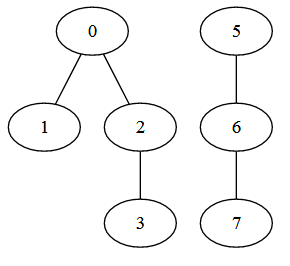
\includegraphics[width=\textwidth]{imgs/graph.PNG}
    \caption{Graphe original, non orienté}
  \end{minipage}
  \hfill
  \begin{minipage}[b]{0.4\textwidth}
    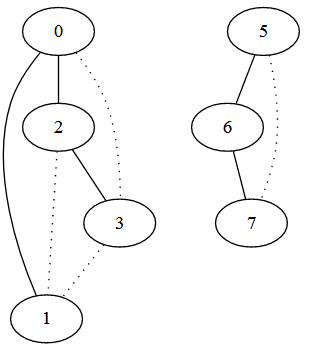
\includegraphics[width=\textwidth]{imgs/graphFT.PNG}
    \caption{Graphe et sa fermeture transitive}
  \end{minipage}
\end{figure}

\iffalse
Code du graphe (enlever les dotted pour le graphe original)

graph G {
	0 -- 1
    0 -- 2
    2 -- 3
    5 -- 6
    6 -- 7
    3 -- 1 [style=dotted]
    5 -- 7 [style=dotted]
    2 -- 1 [style=dotted]
    0 -- 3 [style=dotted]
}
\fi

On va attribuer à chaque chemin une valeur de confiance ou score de confiance qui va déterminer si ce chemin peut être utilisé pour évaluer un fait. Ce score va d'abord dépendre du degré (liens avec d'autres entités) des noeuds traversés. Une entité générique aura un degré important ce qui diminuera le score de confiance, ex : un pays, une grande organisation, etc. D'un autre côté ce score sera plus élevé s'il traverse des noeuds moins génériques, ex : personne, livre, etc. En effet un lien entre deux entités sera plus pertinent si le chemin ne traverse que des entités avec peu de relations et le contexte sémantique sera plus précis. En suivant la même logique lorsque deux entités sont directement liées, on va leur accorder un score de confiance maximal : il n'y a pas d'intermédiaires.

Le chemin qui aura le score le plus élevé sera le chemin le plus court et qui traversera les entités les moins générique. C'est ce que l'on va appeler la proximité sémantique. Cette proximité sémantique représente le sens qui relie deux entités. Pour un fait donné, est-ce que c'est deux entités mise bout à bout ont du sens ? 

Pour le moment nous avons vu comment choisir un chemin entre deux entités, qui va nous permettre ensuite de déterminer si un fait est vrai ou faux. 
\\*
Pour illustrer ceci, prenons un exemple, soit des faits qui lient des villes avec des pays. Pour chaque pays et chaque villes on va tester l'assertion : \enquote{La capitale du pays x est y}.

\begin{figure}[h]
\centering
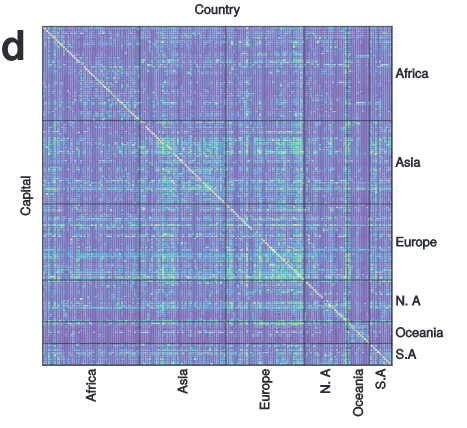
\includegraphics[draft=false, scale=0.5]{imgs/country_cap_check.PNG}
\caption{Pays et capitales groupées par continent}
\label{fig1}
\end{figure}

\todo{\url{http://www.kurzweilai.net/a-computational-algorithm-for-fact-checking}}

Plus un point est clair et plus le fait a de chance d'être vrai. Le chemin entre un pays et sa capitale possède une proximité sémantique plus forte que le chemin entre un pays et n'importe quelle autre ville. Bien que cette méthode soit très basique, elle apporte des résultats satisfaisant. Le taux de réussite selon les datasets utilisés varie entre 61\% et 95\%. Cet exemple prouve que le fact checking peut se faire au travers de graphes de connaissances. 

\paragraph{Critique} Cette méthode permet de faire du fact checking sur des faits simples. Elle se fait entre deux entités clairement définies. Le champs des possibles pour les faits à vérifier est donc limité.

Problème de scalabilité, important d'avoir le verdict instantanément.

Nous verrons plus tard, avec des méthodes plus avancées, certains problèmes inhérents à l'utilisation de KG pour le fact checking.

Ciampaglia et al. [8] propose
an approach that relies on a single short, specific path to
differentiate a true fact from a false one. Although intuitive,
their algorithm fails to account for the semantics of the target
predicate

\todo{Ouvrir sur la seconde approche knowledge stream et montrer qu'il améliore cette approche}

\todo{A lire : https://searchengineland.com/google-researchers-introduce-system-rank-web-pages-facts-not-links-215835}
\label{sec:wkg}

\subsection{Fact checking à base de réseaux de flots} 

Nous avons vu que le fact checking de faits simples était possible via le parcours d'un graphe de connaissance. Seulement plusieurs problèmes peuvent se poser comme la montée en charge d'une telle approche ou sa fiabilité. Dans ce papier, une nouvelle approche est utilisée pour organiser et parcourir un graphe de connaissance. Le code source est disponible \href{https://github.com/shiralkarprashant/knowledgestream}{ici}.

\begin{wrapfigure}{r}{0.5\textwidth}
  \begin{center}
    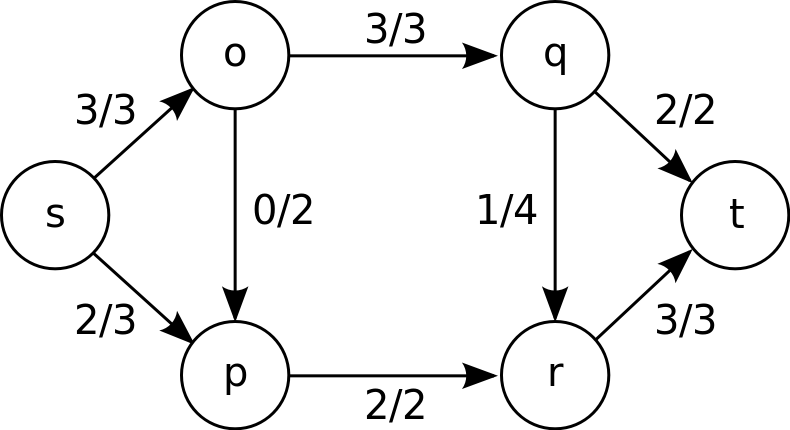
\includegraphics[width=0.6\textwidth]{imgs/max_flow.png}
  \end{center}
  \caption{Graphe/Réseau de flot non orienté}
  \label{max_flow}
\end{wrapfigure}

Cette approche consiste à organiser un graphe comme un réseau de flot \cite{shiralkar2017finding}. Dans un réseau de flot, chaque arête possède une capacité maximale dans laquelle peut passer un flux. Avec cette approche on va chercher à évaluer sémantiquement chaque chemin allant d'une entité A vers une entité B. Plusieurs chemins vont apporter plusieurs contextes qui vont permettre d'évaluer sémantiquement le fait. En outre, la recherche de chemins optimaux est limité par la capacité maximale de chaque arête. 
\\*
En travaillant sur un réseau de flot et en contraignant ainsi chaque flux, on réduit le nombre de chemins possibles entre deux entités. De plus on limite le nombre d'arêtes communes entre chaque chemin. On a ainsi des chemins plus variés en terme de contexte sémantique. Dans la figure \ref{max_flow}, pour aller de s vers t il est possible de passer par l'arête p \textrightarrow r, sans contraintes, l'algorithme passera toujours par cette arête. L'espace restreint va l'obliger à passer par o \textrightarrow q et ainsi fournir de nouvelles informations.
\\*
Ces chemins vont construire l'argumentaire sur lequel le système va s'appuyer pour rendre un verdict sur le statut d'un fait.

\begin{figure}[H]
\centering
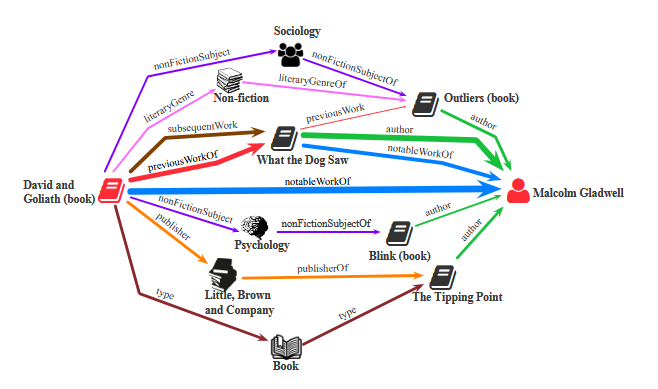
\includegraphics[width=\textwidth, draft=false]{imgs/bookAuthorKG.PNG}
\caption{Relations entre un livre et son auteur dans un graphe de connaissance \cite{shiralkar2017finding}}
\label{stream}
\end{figure}

La figure \ref{stream} représente l'argumentaire autour du triplet t = (David and Goliath (book), author, Malcolm Gladwell). Plus une arête est directe et plus elle est épaisse. Plus elle est épaisse et plus le flux d'informations est important. Cela permet de privilégier les chemins courts dans lesquels les informations contenues sont sémantiquement importantes. 
\\*
Pour un triple donné (s, p, o) il faut voir l'information comme une quantité abstraite qui doit voyager du sujet s vers l'objet o. Chaque arête possède une capacité permettant de transporter plus ou moins d'informations, mais aussi un coût d'utilisation. Ce coût d'utilisation représente le coût d'envoi d'une unité d'information sur le réseau. Ce coût d'utilisation permet encore de s'assurer que les chemins seront le plus court et spécifique possible.
\\*
Le but est donc de trouver les chemins pour lesquelles nous pouvons transporter le plus d'informations entre s et o pour un coût minimal.

\paragraph{Fact checking dans un réseau de flot}

Nous allons voir à présent deux méthodes de fact checking qui appliquent ce concept de réseau de flot dans un graphe de connaissance : Knowledge Stream et Relational Knowledge Linker. Ces méthodes vont construire l'argumentaire d'un fait autour des relations entre les triples qui composent un chemin.

\subsubsection{Knowledge Stream}
\label{sec:ks}

\paragraph{Analogie entre les relations}

Afin de construire un contexte qui va être le plus proche possible de celui du fait énoncé, on va déterminer les relations homologues entre celle du fait et celles existantes dans notre KG. Par exemple pour déterminer l'auteur d'un livre on ne va pas aller regarder les relations concernant l'architecture mais bien celles concernant la littérature.

Pour évaluer l'analogie entre les relations on va construire un graphe G dans lequel les sommets sont des entités et les arêtes des relations. Dans la figure \ref{graph_g},  entre les entités A et C on a une relation de type c (qui peut être par exemple une relation de type \enquote{est marié à}).
\\*
La figure \ref{linear_g_graph} représente le graphe adjoint de G. Par définition, étant donné un graphe G non orienté, le graphe adjoint de G, noté L(G), est un graphe qui représente la relation d'adjacence entre les arêtes de G. Ainsi chaque sommet de L(G) représente une arête de G. Deux sommets de L(G) sont adjacents si et seulement si les arêtes correspondantes partagent une extrémité commune dans G \cite{wiki:lg}.
\\* 
Dans la figure \ref{linear_g_graph} on peut voir que certains noeuds sont représentés plusieurs fois comme a1 et a2 alors qu'ils définissent la même relation. Pour palier à ce problème il faut contracter le graphe comme dans la figure \ref{w_line_graph}. On fusionne chaque sommet commun et on pondère les arêtes en fonction des relations précédentes des sommets.
\\*
Cette démarche va nous permettre de définir les similarités entre les relations. Les arêtes pondérées dans la figure \ref{w_line_graph} représentent la fréquence à laquelle chaque relation co-incident avec ses voisins dans G. Plus cette pondération est importante et plus la similarité entre les relations est forte.

Au final, à partir de la matrice d'adjacence du graphe contracté, on va pouvoir établir des corrélations entre les différentes relations (ici les sommets) à l'aide du TF-IDF (term frequency-inverse document frequency). Cette méthode va évaluer l'importance d'une relation au sein du graphe. Déterminer l'importance d'une relation va nous permettre d'établir un contexte plus précis pour un fait donné. 

\iffalse
Code du graphe G original

graph G {
    A -- B  [label="a1"];
    A -- C  [label="c"];
    A -- D  [label="a2"];
    B -- C  [label="b"];
    C -- E  [label="e1"];
    C -- F  [label="f"];
    D -- E  [label="d"];
    E -- F  [label="e2"];
}

G linear graph

graph G {
    a1 -- a2
    a1 -- c
    a1 -- b
    a2 -- d
    a2 -- c
    b -- c
    b -- e1
    b -- f
    c -- e1
    c -- f
    d -- e1
    d -- e2
    e1 -- e2
    e1 -- f
    e2 -- f
}

Weighted G linear graph

graph G {
    a -- b [label="1"];
    a -- c [label="2"];
    a -- d [label="1"];
    b -- c [label="1"];
    b -- e [label="1"];
    b -- f [label="1"];
    c -- e [label="1"];
    c -- f [label="1"];
    d -- e [label="2"];
    e -- f [label="2"];
}
\fi

\begin{figure}[H]
  \centering
  \begin{minipage}[b]{0.3\textwidth}
    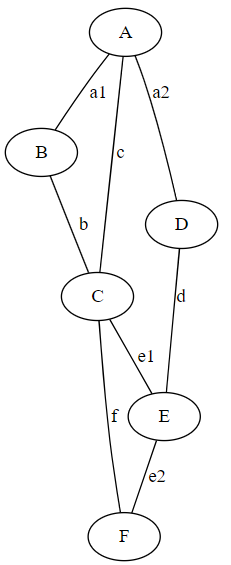
\includegraphics[width=\textwidth]{imgs/graph_g.PNG}
    \caption{Graphe G original, non orienté}
    \label{graph_g}
  \end{minipage}
  \hfill
  \begin{minipage}[b]{0.3\textwidth}
    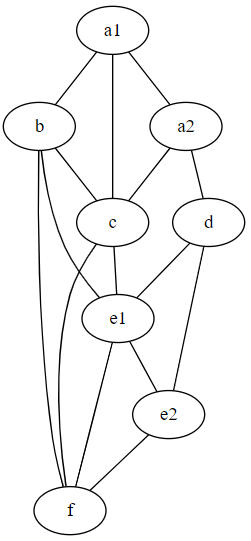
\includegraphics[width=\textwidth]{imgs/linear_g_graph.PNG}
    \caption{Graphe adjoint G'}
    \label{linear_g_graph}
  \end{minipage}
  \hfill
  \begin{minipage}[b]{0.3\textwidth}
    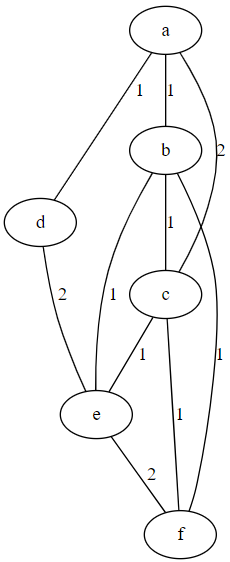
\includegraphics[width=\textwidth]{imgs/w_line_graph.PNG}
    \caption{Graphe adjoint contracté G*}
    \label{w_line_graph}
  \end{minipage}
\end{figure}

\paragraph{Problème de minimisation dans un réseau de flot}

Pour rappel nous cherchons à trouver l'ensemble des chemins pour lesquels le flux maximum est poussé de s vers o pour un coût minimal. Un réseau de flot vient avec différentes contraintes. Il faut tout d'abord pouvoir déterminer la pondération des relations entre les entités, savoir combien d'unités d'information je peux passer d'une entité à une autre. Pour cela on va se baser sur le calcul précédent qui détermine la similarité entre les relations. La quantité disponible pour chaque flux sera calculé selon la similarité avec le prédicat du triplet cible. Plus deux relations seront similaires et plus le flux alloué sera important. En outre, plus un fait sera général (plus il aura de relations), moins son flux sera important.

Une autre contrainte énoncée plus haut est le coût d'utilisation du réseau, chaque chemin à un coût. On cherche à minimiser ce coût et dans cette approche minimiser le coût signifie traverser le moins d'entités génériques possible. Les entités trop génériques ne permettent pas de récupérer des informations précises dans un contexte donné. Le coût d'utilisation d'une arête sera donc déterminé par les relations de ses sommets avec les sommets adjacents.

La dernière contrainte est que dans un réseau de flot, le flux entrant dans un sommet doit être égal à son flux sortant. Il faut pouvoir déterminer le flot maximum qui peut être envoyé entre s et o.
\\*
Cette contrainte est représentée ainsi :
\begin{equation}
   \sum\limits_{P_{s,p,o}  \in  \mathcal{P}_{s,p,o}}  \beta(P_{s,p,o})
\end{equation}

Où $ \beta(P s,p,o) $ représente le plus petit flot possible pour un chemin. Il s'agit de l'arête qui possède la capacité minimale sur un chemin. Les unités d'informations que je peux envoyer sur un chemin seront limitées par $ \beta(P s,p,o) $. Dans cette approche, cette arête représente le triple le moins pertinent pour notre chemin.
\\*
Si on reprend la figure \ref{max_flow}, on ne pourra jamais envoyer plus de 5 unités d'informations de s vers t. En effet les chemins qui mènent vers t sont limités. Si entre o et q mon flot maximum était de 2, alors je ne pourrais jamais envoyer plus de 4 unités d'informations de s vers t. Donc l'information maximale que je peux envoyer se calcul à partir de la somme des capacités minimales de chaque chemins allant de s vers t. Soit la somme des $ \beta(P s,p,o) $.

Au final, sachant que je peux envoyer x unités d'information sur mon réseau, comment maximiser les informations viables que je peux récupérer ? Pour cela il faut pouvoir déterminer des chemins spécifiques pour éviter les chemins trop génériques. Ex : si mon chemin passe par l'entité \enquote{France} on va lui attribuer une faible valeur sémantique. On solutionne ce problème par la contrainte suivante :

\begin{equation}
   \mathcal{S}(P_{s,p,o}) = \frac{1}{1 + \sum\limits_{i=2}^{n-1} \log k(v_{i})}
\end{equation}

Où $ k(v_{i}) $ représente le degré du noeud $ v_{i} $. On va établir un score sémantique déterminé par la somme des degrés des noeuds (nombre de relations) en relation avec $ P_{s,p,o} $. Plus $ P_{s,p,o} $ aura de relations et plus il aura de relations génériques, moins son score sémantique sera élevé.

Ainsi nous allons pouvoir établir un score de fiabilité pour un triple :
\begin{equation}
   \beta(P_{s,p,o}) \times \mathcal{S}(P_{s,p,o})
\end{equation}

Pour un triple donné, son score de fiabilité sera évalué par le produit entre le flot maximum que peut porter le chemin et le score sémantique du triple. Pour rappel, plus un triple est direct et plus son flot maximum est élevé. Un triple avec un score élevé sera court, le plus direct possible, et aura peu de relations avec des entités génériques. Finalement, pour évaluer le score de fiabilité d'un chemin, il suffit de sommer tous les scores de fiabilité des triples qui le compose.

\subsubsection{Relational Knowledge Linker}

Cette approche cherche à étendre des méthodes de fact checking sur des graphes de connaissance déjà existants.
Pour l'approche précédente on se concentre sur la sémantique du sujet et de l'objet, on favorise le sens que l'on peut tirer du triple. L'argumentaire se construit autour de la spécificité de chaque triple.
\\*
Dans cette approche on va se concentrer sur la similarité entre les relations qui lient l'objet et le sujet pour construire notre argumentaire. On se base sur la sémantique du prédicat. Ainsi on va chercher à maximiser la sémantique autour des relations entre les triples. Cette approche étend ce que nous avons vu dans la section \ref{sec:wkg} en y ajoutant la similarité entre les relations.

\subsubsection{Critique}

L'évaluation de cette approche s'est faite sur des datasets déjà formatés, des triples issus notamment du Google Relation Extraction Corpora
(disponible \href{https://github.com/google-research-datasets/relation-extraction-corpus}{ici}). Aucune application dans la vie réelle n'a été conduite. Pour des cas d'application réels il faut pouvoir vérifier un fait en langage naturel. Pour cela il faut pouvoir identifier dans un fait, et avec certitude, les deux entités et la relation qui les unit. On en revient à un problème de TALN. Comment je vais fournir à mon système des données qu'il peut traiter ? On peut envisager plusieurs méthodes pour palier à ce problème, les faits devant être simples, on peut utiliser le TALN ou le machine learning \cite{googleai}. On ne peut pas simplement analyser chaque mot et le comparer avec les données présentes dans le graphe. C'est possible pour identifier les entités, mais pour ce qui est des relations il y a toujours plusieurs façons d'exprimer un même lien.

Pour rappel, cette approche permet de faire du fact checking sur des faits de la forme d'un triplet. Soit des faits simples. Et bien que les faits soient simples, le temps pour vérifier un seul fait se calcul selon une complexité pseudo-polynomiale. Soit $ O(Y|E|\log |V|)$ où V représente les sommets du graphe, E les arêtes et Y le flot maximum d'informations que l'on peut faire passer sur le réseau. Sur des graphes géants tels que DBPedia on obtient un temps moyen (sur laptop) de 356 secondes pour la vérification d'un fait. On peut s'interroger sur l'utilité d'une telle approche pour vérifier des faits en live ou même pour servir d'outil pour aider les journalistes. Avec cette approche la complexité va grandissante en fonction de la taille du graphe. Travailler sur des graphes complets, qui bénéficient de grandes quantités d'informations peut demander beaucoup de temps. Le graphe utilisé pour conduire les expériences est issu des infobox de wikipédia et est constitué de 6 millions d'entités donnant 24 millions de triples déterminés par 663 relations différentes. En comparaison, wikidata est constitué de plus de 48 millions d'entités \cite{wikidata:statistics} \cite{wikidata:statistics2} et le Google Knowledge Graph de plus de 500 millions d'entités et 3.5 milliards de faits à leur sujet \cite{google:kg}.

Pour une montée en charge il faut pouvoir réduire ce temps de calcul. Pour cela il faudrait pouvoir abroger ou du moins anticiper le caractère unique de chaque fait. En effet, pour un fait a traiter, il faut reproduire toutes les étapes vues précédemment. Il est impossible de réutiliser des données calculées en amont, sur d'autres faits, pour réduire le temps de calcul. En effet, pour chaque fait le graphe se modélise de façon unique. Pour chaque fait les entités et relations en cause ne seront pas les mêmes. Il est donc nécessaire de reconstruire le graphe.

Une autre limitation est la rareté de la donnée. Bien que les bases de connaissances existantes soient immenses, elles ne sont pas comparables au flux de données quotidien qui transite sur internet. De plus les bases de connaissances comme Wikidata ou DBPedia ne contiennent aucune news ou informations récentes. Pour DBPedia on ne pourra vérifier un fait que si l'information est présente dans wikipédia. D'autre part, si ce manque de données venait à être résolu on se retrouverait avec des graphes tellement grands qu'il serait impossible de les analyser dans des temps raisonnables avec les méthodes présentées.


\subsection{Conclusion}

Nous avons vu que les KG permettent de réaliser des opérations de fact checking sur des faits simples dans des temps plus ou moins raisonnables. Du fait du manque de données et de la complexité des faits à analyser il est difficile de penser à un système de fact checking entièrement autonome à base de KG. Le temps de calcul est aussi un frein important. En revanche cette approche nous apporte des informations essentielles pour les autres méthodes et système de fact checking : un contexte sémantique. Ce contexte sémantique se matérialise par la construction de l'argumentaire d'un fait qui évalue son environnement et confronte ses liens avec l'existant. Pour ClaimBuster par exemple cela permettrait d'ajouter du sens à l'information et ainsi améliorer sa recherche d'informations permettant de contextualiser le fait.

D'autre part il est possible d'étendre cette approche vers des modèles de statistiques prédictives pour palier à ce manque de scalabilité \cite{wilcke2017knowledge}. C'est-à-dire analyser des faits présents et passés pour faire des hypothèses sur des événements futurs. Appliqué au machine learning il serait possible d'entraîner le système au fil des requêtes pour améliorer le temps de construction du graphe associé aux similarités entre les relations et appliquer un verdict sur un fait plus rapidement. Il est aussi possible de construire un argumentaire qui s'étendrait sur plusieurs faits, c'est-à-dire traiter un fait comme étant en relation avec d'autres faits. Ainsi il serait possible de construire une cohérence dans un texte entre les faits analysés.

Pour réaliser une approche par les graphes de connaissances il est possible de faire appelle à des apis, notamment celle du Google Knowledge Graph (GKG) ou Unigraph. Le GKG est ce qui permet au moteur de recherche de Google d'ajouter de la sémantique aux résultats d'une requête. Il est possible pour des faits simples et corrélés de trouver un lien déterminant pour assurer un verdict. Par exemple, il est possible de résumer la méthode précédente à une simple requête et à l'analyse syntaxique de la réponse. Si on prend l'assertion suivante : \enquote{Joseph Boyden wrote Three Day Road}. Si on recherche sur l'api les deux entités, on va tout de suite établir le lien entre elles. En annexe sont disponibles les fragments importants retournés par l'api (\ref{appendix:gkg_jb}). 

Enfin, les KGs sont importants pour les modèles qui se reposent sur le machine learning. Ils apportent de la donnée structurée, contextualisée et compréhensible pour la machine. Aujourd'hui, les algorithmes de type machine learning sont entraînés avec de la donnée la plus pure et brute possible. Fournir à ces algorithmes des données plus sophistiquées pourrait permettre de construire des systèmes plus intelligents \cite{nickel2016review}. Cela permettrait en outre de réduire les temps de travail nécessaires pour chaque requête.

Enfin le plus gros manque pour les KGs se trouvent autour de la données. Il y a trop peu de données pour traiter des informations spécifiques. Plusieurs options sont possibles : enrichir les KGs avec des données fiables et à jour automatiquement ou simplement utiliser les sources du web. Dans les deux cas c'est la fiabilité de la source qui sera déterminante.

\subsection{Délégation aux apis}

Faire du fact checking via différentes apis. (voir fib)
https://github.com/anantdgoel/HackPrincetonF16 : exemple avec pas mal d'api

\subsection{Falsification d'image}

Ex : test sur donald trump qui tient la main du pape

https://www.stopfake.org/en/13-online-tools-that-help-to-verify-the-authenticity-of-a-photo/

https://arxiv.org/pdf/1801.02768.pdf : Fake Colorized Image Detection

Regarder la date d'existance de l'image sur google et la confronter avec la date de l'article.

\todo{https://www.letemps.ch/sciences/twitter-mensonge-se-diffuse-plus-vite-plus-loin-verite : Par exemple, «il y a plusieurs moyens de détecter si une image a été falsifiée», indique Ewa Kijak.}


\subsection{Vérification de la source du lien}

Baser la réputation d'un site sur son contenu au fur et à mesure des vérifications (rapport entre fake news/vraies news/news non vérifiées)

\subsection{Développement prototype}

Prototype sur l'analyse de fausses images ? 
Construire un score de confiance.
https://wit.ai/ : NLP (pas forcément utile mais intéressant)
https://github.com/anantdgoel/HackPrincetonF16 : exemple avec pas mal d'api

\subsubsection{Prédire la tromperie}

\cite{conroy2015automatic} voir les citations de ce papier

\subsubsection{A faire}

\todo{Lire : http://nlp.fast.ai/classification/2018/05/15/introducting-ulmfit.html}
\todo{Lire : \url{https://ai.googleblog.com/2013/04/50000-lessons-on-how-to-read-relation.html} et \url{https://github.com/google-research-datasets/relation-extraction-corpus/blob/master/20131104-date_of_birth.json}}
\todo{credeye : \cite{popat2018credeye}}

- Parler de mon expérience dans l'analyse sémantique de texte

A rechercher : 

- Fact checking api
- Computational fact checking 

Prendre le cas de FiB et expliquer pourquoi il est mauvais ?

\clearpage

\printbibliography[
heading=bibintoc,
title={Bibliographie}
]

\clearpage

\begin{appendices}

\section{Knowledge Graph}
\subsection{Fragment du résultat retourné par le google knowledge graph pour l'entité \enquote{Joseph Boyden}}
\label{appendix:gkg_jb}

\begin{lstlisting}
{
 "@context": {
  "@vocab": "http://schema.org/",
  "goog": "http://schema.googleapis.com/",
  "EntitySearchResult": "goog:EntitySearchResult",
  "detailedDescription": "goog:detailedDescription",
  "resultScore": "goog:resultScore",
  "kg": "http://g.co/kg"
 },
 "@type": "ItemList",
 "itemListElement": [
  {
   "@type": "EntitySearchResult",
   "result": {
    "@id": "kg:/m/08gyww",
    "name": "Joseph Boyden",
    "@type": [
     "Thing",
     "Person"
    ],
    "description": "Canadian novelist",
    "image": {
     "contentUrl": "http://t2.gstatic.com/images?q=tbn:
     ANd9GcRXyYM8YrpcumM2NqJZlL5WlNncJYOgUlO-w93ztUOdOJiPK0rV",
     "url": "https://en.wikipedia.org/wiki/Joseph_Boyden"
    },
    "detailedDescription": {
     "articleBody": "Joseph Boyden CM is a Canadian novelist and short 
     story writer. His first novel, Three Day Road, won the 
     Amazon/Books in Canada First Novel Award and the Rogers Writers' 
     Trust Fiction Prize. ",
     "url": "https://en.wikipedia.org/wiki/Joseph_Boyden",
     "license": "https://en.wikipedia.org/wiki/Wikipedia:Text_of_
     Creative_Commons_Attribution-ShareAlike_3.0_Unported_License"
    }
   },
   "resultScore": 428.041321
  },
  {
   "@type": "EntitySearchResult",
   "result": {
    "@id": "kg:/m/0cwbmj",
    "name": "Three Day Road",
    "@type": [
     "Book",
     "Thing"
    ],
    "description": "Novel by Joseph Boyden",
    "detailedDescription": {
     "articleBody": "Three Day Road is the first novel from 
     Canadian writer Joseph Boyden.",
     "url": "https://en.wikipedia.org/wiki/Three_Day_Road",
     "license": "https://en.wikipedia.org/wiki/Wikipedia:Text_of_
     Creative_Commons_Attribution-ShareAlike_3.0_Unported_License"
    }
   },
   "resultScore": 13.805716
  },
  {
   "@type": "EntitySearchResult",
   "result": {
    "@id": "kg:/g/11bw4txn3g",
    "name": "Al Purdy Was Here",
    "@type": [
     "Movie",
     "Thing"
    ],
    "description": "2015 film",
    "url": "http://alpurdywashere.com/"
   },
   "resultScore": 13.146592
  }
\end{lstlisting}

\subsection{Fragment du résultat retourné par le google knowledge graph pour l'entité \enquote{Three day road}}

\begin{lstlisting}
{
 "@context": {
  "@vocab": "http://schema.org/",
  "goog": "http://schema.googleapis.com/",
  "EntitySearchResult": "goog:EntitySearchResult",
  "detailedDescription": "goog:detailedDescription",
  "resultScore": "goog:resultScore",
  "kg": "http://g.co/kg"
 },
 "@type": "ItemList",
 "itemListElement": [
  {
   "@type": "EntitySearchResult",
   "result": {
    "@id": "kg:/m/0cwbmj",
    "name": "Three Day Road",
    "@type": [
     "Book",
     "Thing"
    ],
    "description": "Novel by Joseph Boyden",
    "detailedDescription": {
     "articleBody": "Three Day Road is the first novel from 
     Canadian writer Joseph Boyden. Joseph's maternal 
     grandfather, as well as an uncle on his father's side, 
     served as soldiers during the First World War, 
     and Boyden draws upon a wealth of family narratives.",
     "url": "https://en.wikipedia.org/wiki/Three_Day_Road",
     "license": "https://en.wikipedia.org/wiki/Wikipedia:
     Text_of_Creative_Commons_Attribution-ShareAlike_3.0
     _Unported_License"
    }
   },
   "resultScore": 486.23822
  }
\end{lstlisting}

\end{appendices}

\end{document}
